\section{Экспериментальное исследование}\label{sec:experiments}
\subsection{Данные и протокол}
Основная серия включает шесть наборов данных: числовые измерения, изображения цифр и тексты (табл.~\ref{tab:datasets}). Для каждого набора фиксируются одна подвыборка, набор разбиений и разделение на резерв и проверочную часть. Признаки всех объектов доступны при кластеризации. Проверочные метки скрыты до фиксации решений.

\begin{table}[t]
\centering
\caption{Наборы основной серии. Для текстов размерность 50 получается после проекции векторных представлений MiniLM методом главных компонент.}
\label{tab:datasets}
\begin{tabular}{lrrl}
\toprule
Набор & Объектов & Классов & Признаки для кластеризации\\
\midrule
Breast Cancer & 569 & 2 & 30 стандартизированных измерений\\
Dry Bean & 600 & 7 & 16 стандартизированных измерений\\
Digits & 600 & 10 & 64 стандартизированные яркости\\
AG News & 600 & 4 & 50 главных компонент текстовых векторов\\
20 Newsgroups & 600 & 20 & 50 главных компонент текстовых векторов\\
Banking77 & 600 & 77 & 50 главных компонент текстовых векторов\\
\bottomrule
\end{tabular}
\end{table}

Числовые признаки стандартизированы. Тексты представлены нормированными векторами all-MiniLM-L6-v2 и 50 компонентами PCA. Кластеризация и silhouette используют одно пространство с евклидовым расстоянием. Кандидаты получены KMeans с $k=2,4,8,16$ и спектральной кластеризацией с $k=4,8$. После объединения совпадений на каждых данных остаётся шесть разбиений. Параметры подготовки и алгоритмов приведены в приложении.

На каждом наборе выполнены 20 случайных раскрытий без возвращения с бюджетами 20 и 50 меток. В пределах повтора меньший бюджет входит в больший. Всего рассмотрены 240 условий разметки. Все правила сравниваются на общих раскрытиях. M6 и M7 используют общие 100 парных перевыборок. Расчёты выполнены на CPU.

Для каждого раскрытия рассчитывается разность проверочных ARI выбранных разбиений. Усреднение этих парных разностей даёт эффект при фиксированных признаках, кандидатах и проверочной части. Дополнительно учитываются число переключений и доли улучшений и ухудшений. Такой протокол отделяет случайность раскрытия меток от различий между самими наборами данных. Вложенные бюджеты позволяют сопоставить выбор при добавлении меток в пределах одного повтора.

M0 выбирает максимум silhouette. M1 максимизирует частичный ARI. M2 разрешает равенства ARI по silhouette с численным допуском $10^{-12}$. M5 допускает отставание до $0{,}05$ ARI, затем максимизирует silhouette. M6 использует~\eqref{eq:adaptive}. M7 выбирает по частоте бутстрепных побед. Если в перевыборке несколько кандидатов имеют максимальный ARI с точностью до $\varepsilon$, её голос делится между ними поровну:
\begin{equation}\label{eq:bootstrap-votes}
 W_b=\{P:A_{L^{(b)}}(P)\ge\max_{P'}A_{L^{(b)}}(P')-\varepsilon\},\qquad
 v(P)=\frac1B\sum_b\frac{\mathbf1\{P\in W_b\}}{|W_b|}.
\end{equation}
M7 максимизирует $v(P)$ с тем же порядком разрешения равенств, что остальные правила. Сравнение с M0 характеризует пользу внешней информации, с M2 --- роль допуска кандидатов с положительным отставанием, с M5 --- отличие от простого постоянного порога. Сравнение с M7 позволяет оценить, улучшает ли silhouette результат сверх использования тех же бутстрепных перевыборок.

\subsection{Сравнение правил}
Таблица~\ref{tab:baselines} представляет абсолютный проверочный ARI. Средний парный выигрыш M6 относительно M1 и его неопределённость показаны на рис.~\ref{fig:domain-gain}. При 20 метках средний выигрыш положителен на пяти наборах. На Dry Bean он отрицателен при обоих бюджетах: все 12 переключений при 20 метках и все пять при 50 метках ухудшают ARI.

\begin{table}[htbp]\centering\small
\caption{Средние проверочные ARI всех шести сравниваемых правил.}\label{tab:baselines}
\begin{tabular}{lrrrrrrr}
\toprule
Набор & $m$ & M0 & M1 & M2 & M5 & M6 & M7\\
\midrule
20 Newsgroups & 20 & $0{,}3377$ & $0{,}3106$ & $0{,}3106$ & $0{,}3163$ & $0{,}3213$ & $0{,}3270$\\
20 Newsgroups & 50 & $0{,}3377$ & $0{,}3220$ & $0{,}3220$ & $0{,}3327$ & $0{,}3377$ & $0{,}3377$\\
AG News & 20 & $0{,}2389$ & $0{,}6115$ & $0{,}6115$ & $0{,}6174$ & $0{,}6247$ & $0{,}6073$\\
AG News & 50 & $0{,}2389$ & $0{,}6562$ & $0{,}6562$ & $0{,}6663$ & $0{,}6663$ & $0{,}6562$\\
Banking77 & 20 & $0{,}1974$ & $0{,}1663$ & $0{,}1814$ & $0{,}1867$ & $0{,}1974$ & $0{,}1974$\\
Banking77 & 50 & $0{,}1974$ & $0{,}1974$ & $0{,}1974$ & $0{,}1974$ & $0{,}1974$ & $0{,}1974$\\
Breast Cancer & 20 & $0{,}6858$ & $0{,}6750$ & $0{,}6750$ & $0{,}6858$ & $0{,}6858$ & $0{,}6750$\\
Breast Cancer & 50 & $0{,}6858$ & $0{,}6822$ & $0{,}6822$ & $0{,}6858$ & $0{,}6858$ & $0{,}6822$\\
Digits & 20 & $0{,}5773$ & $0{,}5462$ & $0{,}5462$ & $0{,}5541$ & $0{,}5736$ & $0{,}5541$\\
Digits & 50 & $0{,}5773$ & $0{,}5687$ & $0{,}5687$ & $0{,}5748$ & $0{,}5773$ & $0{,}5736$\\
Dry Bean & 20 & $0{,}2780$ & $0{,}6234$ & $0{,}6234$ & $0{,}6055$ & $0{,}5531$ & $0{,}6251$\\
Dry Bean & 50 & $0{,}2780$ & $0{,}6308$ & $0{,}6308$ & $0{,}6276$ & $0{,}6202$ & $0{,}6308$\\
\bottomrule\end{tabular}\end{table}

\begin{figure}[t]
\centering
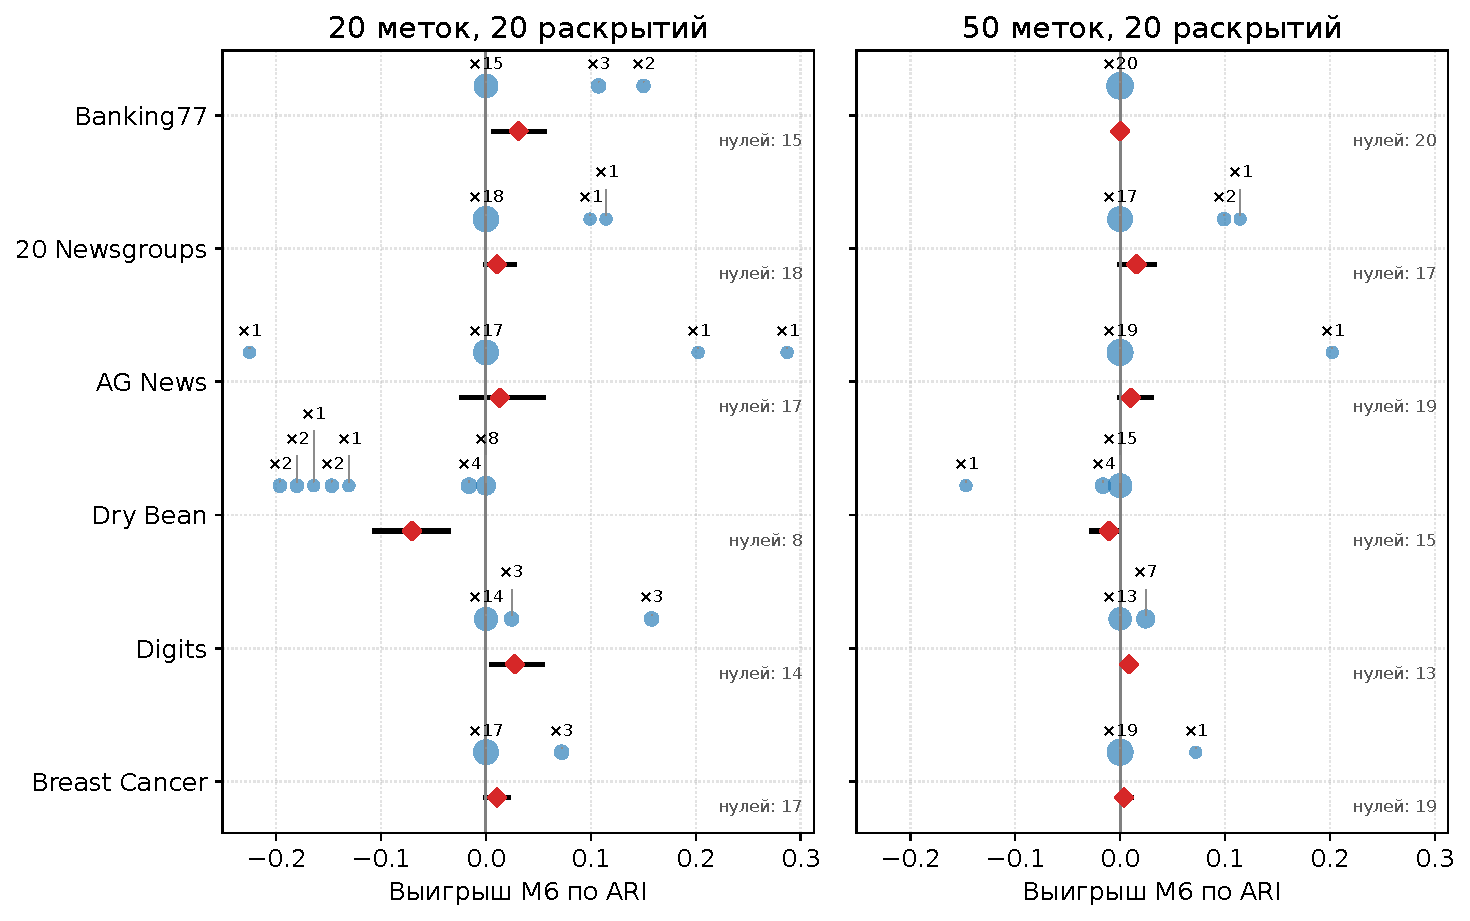
\includegraphics[width=\linewidth]{figures/domain_gain.pdf}
\caption{Эффекты 20 раскрытий с кратностями, средние (ромбы) и условные 95\%-интервалы среднего по перевыборкам раскрытий (отрезки). Фиксированы данные, набор разбиений и проверочная часть. Совпадающие эффекты сгруппированы: площадь маркера и подпись отражают их число. Отдельно указано число нулевых эффектов. Интервалы отражают эмпирическую вариативность наблюдённых раскрытий.}
\label{fig:domain-gain}
\end{figure}

На Digits при 20 метках выигрыш M6 равен $0{,}0273$ ARI против $0{,}0079$ у фиксированного допуска M5. На Banking77 значения равны $0{,}0311$ и $0{,}0204$. На Dry Bean M6 даёт $-0{,}0703$ против $-0{,}0180$ у M5. На Breast Cancer средние эффекты этих правил совпадают при обоих бюджетах. Различие M5 и M6 включает фактическую ширину допуска. Самостоятельная польза адаптации при сопоставимой частоте переключений требует отдельной проверки.

На Banking77, Digits, Breast Cancer и 20 Newsgroups M0 уже выбирает лучший проверочный кандидат. При 20 метках M6 уступает ему на Digits ($0{,}5736$ против $0{,}5773$) и 20 Newsgroups ($0{,}3213$ против $0{,}3377$), поскольку внешний допуск иногда исключает это разбиение. При 50 метках M6 достигает качества M0 на всех четырёх наборах. Такая пригодность геометрического максимума определяется ретроспективно.

На AG News и Dry Bean M0 даёт $0{,}2389$ и $0{,}2780$ ARI. При 20 метках M6 повышает их до $0{,}6247$ и $0{,}5531$. Однако на Dry Bean внешний лидер M1 достигает $0{,}6234$, а M7 --- $0{,}6251$. Выбор по silhouette внутри допуска снижает качество относительно обоих правил. На 20 Newsgroups при 20 метках M6 также уступает M7 на $0{,}0057$ ARI. На Digits и AG News средние парные выигрыши M6 относительно M7 при 20 метках равны $0{,}0195$ и $0{,}0174$ ARI. Следовательно, добавление геометрического выбора к бутстрепному сравнению имеет разный эффект на исследованных данных. Положительный выигрыш относительно M1 следует рассматривать вместе с абсолютным качеством и результатами остальных правил.

\paragraph{Источники потери.}
На Digits и 20 Newsgroups при 20 метках $D_{\mathrm{inside}}=0$. Оставшаяся потеря $0{,}0037$ и $0{,}0164$ ARI возникает при исключении кандидата. На Dry Bean из общей потери $0{,}0875$ на выбор внутри допуска приходится $0{,}0826$, или около 94\%. На AG News обе составляющие близки: $0{,}0202$ при исключении и $0{,}0214$ внутри допуска. Численные разложения приведены в приложении. При 50 метках на Digits, 20 Newsgroups, AG News, Banking77 и Breast Cancer M6 достигает лучшего качества среди кандидатов. На Dry Bean сохраняется потеря, большая часть которой возникает внутри допуска.

На Dry Bean при 20 метках семь переключений меняют число кластеров с восьми на четыре, одно --- с восьми на шестнадцать, четыре сохраняют восемь кластеров. При 50 метках один переход меняет восемь кластеров на четыре, ещё четыре сохраняют восемь кластеров. Ошибки затрагивают как число групп, так и состав разбиений с одинаковым числом кластеров.

\subsection{Контроль целевой группировки}
Сгенерированы четыре группы по 100 точек вокруг центров $(-3,-1)$, $(-3,1)$, $(3,-1)$ и $(3,1)$ с независимым нормальным шумом стандартного отклонения $0{,}2$. Используются три реализации с начальными значениями 101, 102 и 103 без изменения масштабов координат. Целевые классы задаются знаком первой или второй координаты. Кандидаты включают KMeans с двумя, тремя и четырьмя кластерами и правильные разбиения для обеих целей. Между целями сохраняются признаки, разбиения, проверочные объекты, раскрытые индексы и бутстрепные веса.

\begin{figure}[t]
\centering
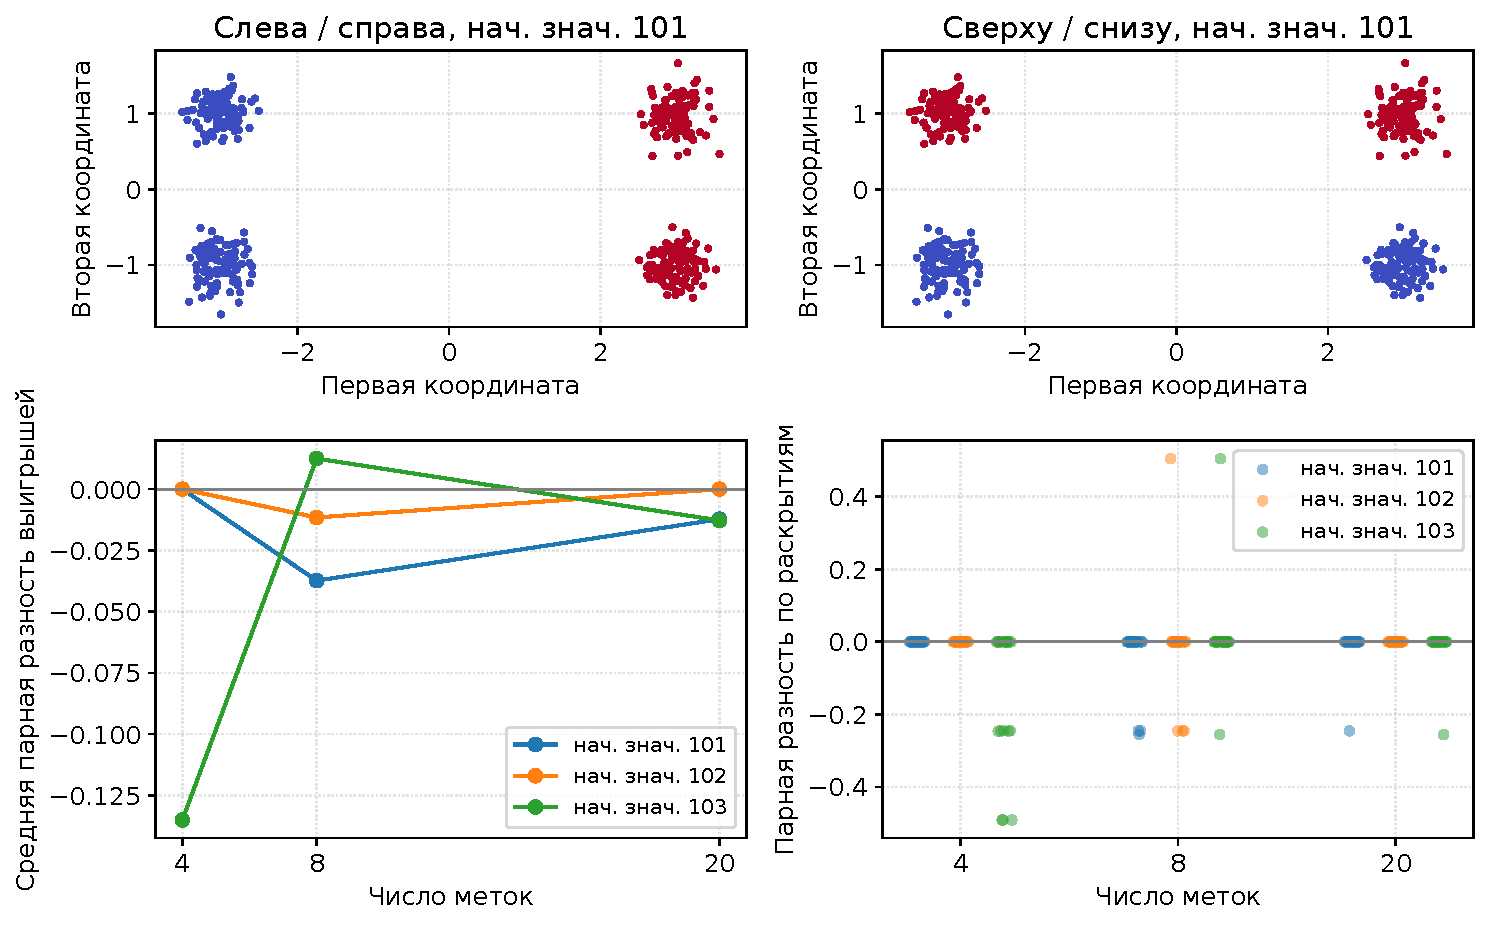
\includegraphics[width=\linewidth]{figures/rectangle_control.pdf}
\caption{Две целевые окраски реализации с начальным значением 101 и парная разность выигрышей $G_{\mathrm{left}}-G_{\mathrm{up}}$. Нижние панели показывают средние отдельно по трём реализациям и эффекты их раскрытий. В каждой реализации 20 раскрытий на бюджет.}
\label{fig:rectangle}
\end{figure}

На каждой реализации выполнены 20 парных раскрытий для бюджетов $4,8,20$. Средняя разность выигрышей $G_{\mathrm{left}}-G_{\mathrm{up}}$ равна $-0{,}0450$, $-0{,}0121$ и $-0{,}0083$ ARI соответственно. Каждый бюджет усредняет 60 пар внутри трёх фиксированных геометрий с одинаковым весом. Эти пары характеризуют раскрытия внутри трёх задач.

Средний silhouette правильного разбиения слева направо равен $0{,}806$, сверху вниз --- $0{,}235$. Для первой цели все 15 переключений ухудшают качество: более дробные разбиения имеют больший silhouette и могут проходить допуск. Поэтому даже высокий silhouette правильного кандидата следует сопоставлять с внутренними оценками остальных альтернатив.

Для цели сверху вниз при четырёх метках есть пять улучшающих переключений, при восьми --- два ухудшающих, при двадцати переключений нет. При четырёх метках средний выигрыш на этой цели равен $0{,}0204$ ARI, тогда как для цели слева направо он равен $-0{,}0246$. При одинаковых признаках и раскрытых индексах эффект зависит от целевой группировки. Этот вывод относится к трём заданным геометриям и двум способам назначения классов.

\subsection{Дополнительные проверки и ограничения}
При неизменных объектах и разметке сравнивались все кандидаты и подмножество KMeans. На AG News при 50 метках выигрыш составляет $0$ и $0{,}0101$ соответственно для подмножества и полного набора, хотя абсолютный ARI M6 в обоих случаях равен $0{,}6663$. Меняется качество M1. На Dry Bean при 20 метках добавление спектральных кандидатов повышает абсолютный ARI M6 с $0{,}5267$ до $0{,}5531$. Одновременно его выигрыш относительно внешнего лидера меняется с $-0{,}0575$ до $-0{,}0703$. Состав кандидатов влияет на оба сравниваемых правила, поэтому изменение относительного выигрыша следует сопоставлять с абсолютными качествами.

При бюджете 20 на Digits и Dry Bean задавались два, четыре или шесть представленных классов. На Digits средний выигрыш меняется с $0{,}0154$ ARI при двух классах до $-0{,}0194$ при шести. На Dry Bean наиболее отрицательный средний эффект наблюдается при четырёх классах. Покрытие, число одноимённых пар, квоты и выбранные категории менялись совместно. Проверка характеризует состав разметки целиком. Независимая монотонная зависимость эффекта от покрытия остаётся неустановленной.

Проверка числа перевыборок охватила все 80 исходных разметок Digits и Breast Cancer. На Digits при 20 метках для каждого $B=30,100,300$ получено 96 совпадений из 100 запусков с ориентиром при $B=3000$. Все несовпадения относятся к двум разметкам и сопровождаются разными потерями ARI. При дополнительной смене начального значения сам ориентир меняет решение в одной разметке. Поэтому одинаковая доля совпадений при разных $B$ требует анализа отдельных случаев около границы допуска. Подробности обеих проверок даны в приложении.

Выводы относятся к одному разделению, одной подвыборке и исходному набору кандидатов для каждых реальных данных. Двадцать повторов оценивают случайность раскрытия меток, интервалы используются описательно. Digits и Breast Cancer рассматривались при разработке процедуры. Дополнительные проверки имеют разведочный характер. Различия представлений, числа и смысла классов ограничивают перенос наблюдений на области применения в целом. Для Banking77 максимум числа кластеров равен 16 при 77 классах, а лучший проверочный ARI составляет $0{,}1974$, что ограничивает качество даже без ошибки выбора.
